\section{Mathematical Model}
\frame{\sectionpage}
\begin{frame}{Model of intraocular fluids dynamics}
\begin{block}{}
\[
\frac{\dd U}{\dd t}=F_{h}-F_{e}
\]
\end{block}
\begin{itemize}
\item $U$: Total aqueous humor
\item $F_h$: Fluid inflow in posterior chamber
\item $F_e$: net outflow via trabecular path
\end{itemize}

\begin{center}
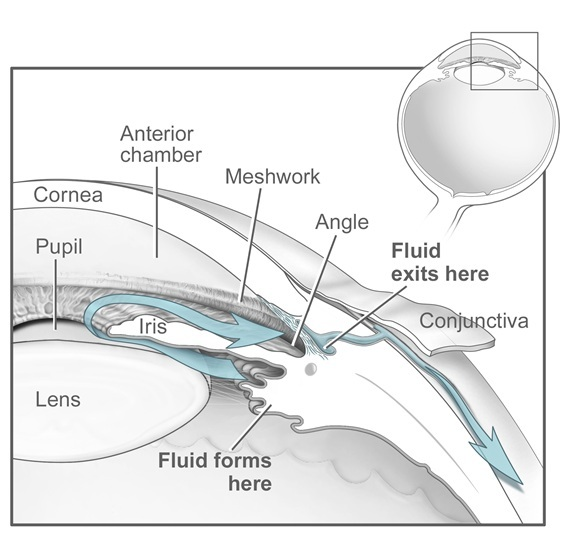
\includegraphics[width=.4\linewidth]{Humor.jpg}
\end{center}

\end{frame}

\begin{frame}{Model of intraocular fluids dynamics}

\[
F_{h}= L_p \big[ (p_a-p)-\sigma_{p} \Delta\pi_{p}-\sigma_{s} \Delta\pi_{s}\big]
\]

\only<1>{
\begin{itemize}
\item $L_p$: permeability of the equivalent membrane
\item $p_a$: pressure in the ciliary body capillaries
\item $p$: IOP
\item $\sigma_p$: reflection coefficient (proteins)
\item $\sigma_s$: reflection coefficient (low molecular components)
\item $\Delta \pi_p $: osmotic pressure diff. accross membrane (proteins)
\item $\Delta \pi_s $: osmotic pressure diff. across membrane (low molecular component)
\end{itemize}}
\only<2>{
\[
\Delta\pi_{s}= \rho(C_1-C_{2})
\]
\begin{itemize}
\item $\rho$: universal gas constant $\times$  absolute temperature
\item $C_1$: total molar concentration of low-molecular components (blood)
\item $C_2$: total molar concentration of low-molecular components (intra-ocular fluid near ciliary body surface)
\end{itemize}
}
\end{frame}

\begin{frame}{Model of intraocular fluids dynamics}
\[
F_{e}= \frac{p - p_e}{R}
\]
\begin{itemize}

\item $p_e$: pressure in the episcleral veins
\item $R$: output hydraulic resistance
\end{itemize}
\end{frame}



\begin{frame}{Stationary case}
\Alert{Assumption :} inflow rate = outflow rate
\begin{block}{}
\[
F_h = L_p \left(p_a-p-\Delta \pi_p - \sigma_s \Delta\pi_s\right) = \frac{p - p_e}{R}, \; \Delta \pi_s = \rho(C_1-C_2)
\]
\[
F_h (1 - \sigma_s) \overline{C} + J = F_hC_2 , \; \overline{C}= C_1+C2
\]

\end{block}
\begin{figure}[H]
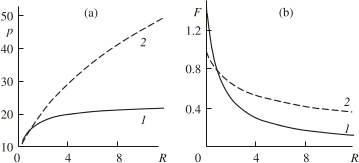
\includegraphics[scale=0.7]{images/courbes_pr_fr}
\end{figure}
%\textcolor{red}{Not clear what are cases 1 and 2}
\begin{center}
\tiny{source : \textit{Dynamic of the intraocular fluid}Lyobimov et al, 2007}
\end{center}
\small{$1$: Purely hydraulic model ($\Delta\pi_s$ is constant)\\
$2$: Osmotic components dynamics ($J$ is constant)}
\end{frame}


\begin{frame}{Nonstationary case}
Linearisation of $V(p)$
\[
V = V(p) \approx V_0 + \alpha (p-p_0)
\]
$\alpha$ : volume compliance of the eye shell (directly measured in experiments/varies significantly)

\begin{block}{}
\[
 \alpha \frac{dp}{dt}=F_{h}-\frac{p-p_e}{R}
 \]
\[
 V^{\ast} \frac{dC_{2}}{dt}= F_h(1-\sigma_s)\overline{C} + J - F_hC_2,\; \overline{C}= \frac{C_1+C_2}{2}
 \]
\begin{center}
+ initial conditions
\end{center} 
\end{block}

$V^\star$: volume of intraocular fluid between the folds of the ciliary body\\
$J$: Influx due to active transport

\end{frame}
